% Chapter on Online Monitoring, Data Quality Monitoring & Event Displays
% 10 pages

\chapter{Online Monitoring \& Event Displays for the 35ton}

Monitoring of the data collected during the running of an experiment is imperative to ensure a high quality of data is maintained.  Such monitoring is often provided in real-time (`Online Monitoring'), summarising the data from the current run, or in near real-time (`Nearline Monitoring'), summarising data over runs from typically the previous day, week or month to represent the longer term fluctuations in the data quality.  An event display, designed to illustrate physics events as they occur in the detector, is another desirable feature hugely useful to those ensuring the smooth running of the data collection.  A basic example of such a display is also produced by the monitoring system for the purposes of ensuring good quality physics data collection is maintained.  The system developed to provide online feedback, including an online event display, for the 35ton Run II data taking period is discussed in this present section.

The system is designed to be flexible and provide prompt feedback for those operating the experiment.  It was thus included as part of the DAQ (Data Acquisition) system, lbne-artdaq, discussed in Sec. \ref{sec:lbne-artdaq}.  The monitoring framework itself is the subject of Sec. \ref{sec:OnlineMonitoring}, with its two functions, data quality monitoring and producing online event displays, presented in Sec. \ref{sec:DQM} and Sec. \ref{sec:EventDisplay} respectively.  Finally, the web interface developed to fascilitate synchronisation of this monitoring data to a dedicated web page for ease of access is briefly described in Sec. \ref{sec:WebInterface}.

\section{The DAQ Framework}\label{sec:lbne-artdaq}

Experiments at FNAL are moving over to using artdaq, a centrally-maintained data acquisition system built on the art framework utilised by all offline software written for experiments hosted at the lab.  The DUNE 35ton experiment was one of the first to use this new software (may be the first... but uBooNE and LArIAT possibly use it... I'll check!) and used an experiment specific system named lbne-artdaq \footnote{Since the formation of the DUNE experiment occurred only a few months before the running of the 35ton, all online software maintained the use of the outdated `lbne' descriptor to prevent unnecessary potential problems associated with large scale code changes and alleviate the risk of further delays.  It should be again stressed that the 35ton was recognised by the DUNE collaboration as an integral part of the DUNE plan and the use of \textit{lbne} was in no way an indication of a project associated only with the dissolved previous experiment!}.  A general overview of lbne-artdaq is shown in Fig. \ref{fig:lbne-artdaq}.

\begin{figure}[ht]
  \centering
  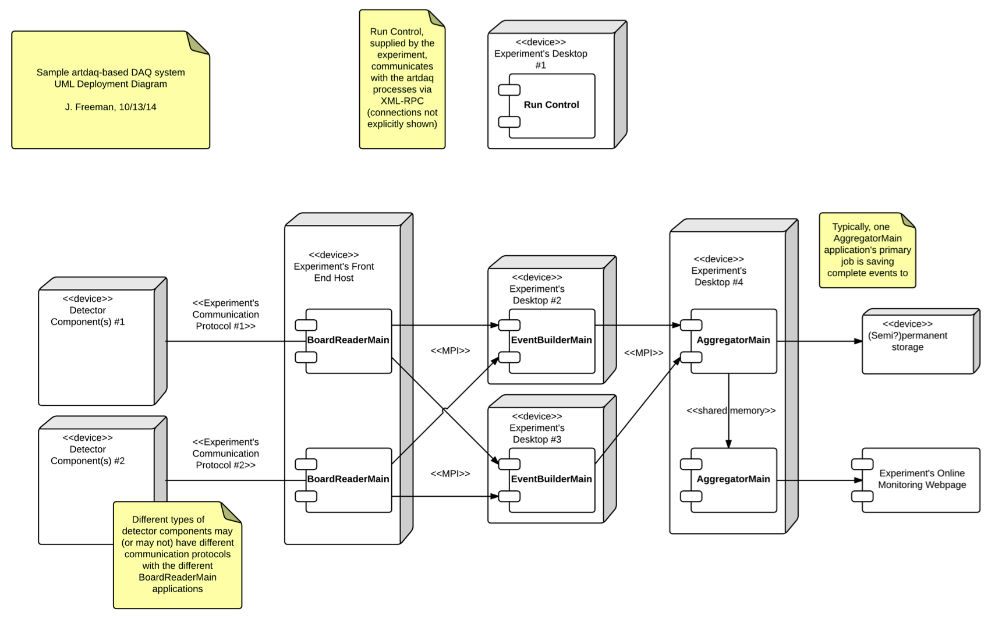
\includegraphics[width=12cm]{lbne-artdaq.png}
  \caption{Overview of the lbne-artdaq framework used for data acquisition by the DUNE 35ton experiment.  See the text for a complete description.  [Thank John Freeman for this image... how to reference?]}
  \label{fig:lbne-artdaq}
\end{figure}

Data flows from left to right and pass through components common to most DAQ systems.  Closest to the detector components (i.e. the RCEs, SSPs and PTB [see Sec. \ref{sec:DetectorComponents}]) are the board readers which take the output from the firmware as soon as it is ready and sends it downstream to the event builders.  There exists a board reader for each of the detector components (totalling 24) and each is unaware of the existence of the others.  It is the job of the event builders to assemble a full `event' from these individual `fragments' passed on from each of the detector elements.  An event is complete once composed of a full set of `\texttt{artdaq::Fragment}s' and the event builders will wait to receive them all before sending the data onwards to the aggregators.

There are two aggregators which take the full events but process them in very different ways.  All the data passes through only the first aggregator, whose function it is to write the output to disk and thus end processing by the DAQ.  The second aggregator receives no events but instead has access to the shared memory occupied by the data as it passes through the first aggregator; it is thus designed specifically for the purpose of monitoring and in no way affects the data or the output from the first aggregator.  It is within this second aggregator process that the online monitoring system described in the proceeding section is designed to run.

Each of the DAQ processes runs on a machine on the private DAQ network and is configured as normal within art (using the \textit{fhicl} (Fermilab Hierarchial Configuration Language) configuration language).  Two nodes on the main FNAL network (lbne-gateway01/02) provide access to these private machines, of which there are 7 (lbnedaq1-7), and contain all scripts and setup necessary to run through the DAQ via a command line interface.

\section{Online Monitoring Framework}\label{sec:OnlineMonitoring}

The framework developed for the monitoring system had the following desgin goals:

\begin{itemize}
\item to be able to analyse the data read out of memory it in its raw `DAQ format`;
\item to be as computationally efficient as possible to allow for processing at the event rate;
\item to provide the flexibility for further monitoring plots to be added with ease;
\item to allow for use of an online event display to provide comprehensible images of the raw data.
\end{itemize}

In general, the final developed system succeeded in all these goals and provided invaluable information, becoming an integral tool in the commissioning and the data taking of the 35ton.  An illustration of the framework is shown in figure \ref{fig:OnlineMonitoringFramework}.

\begin{figure}[ht]
  \centering
  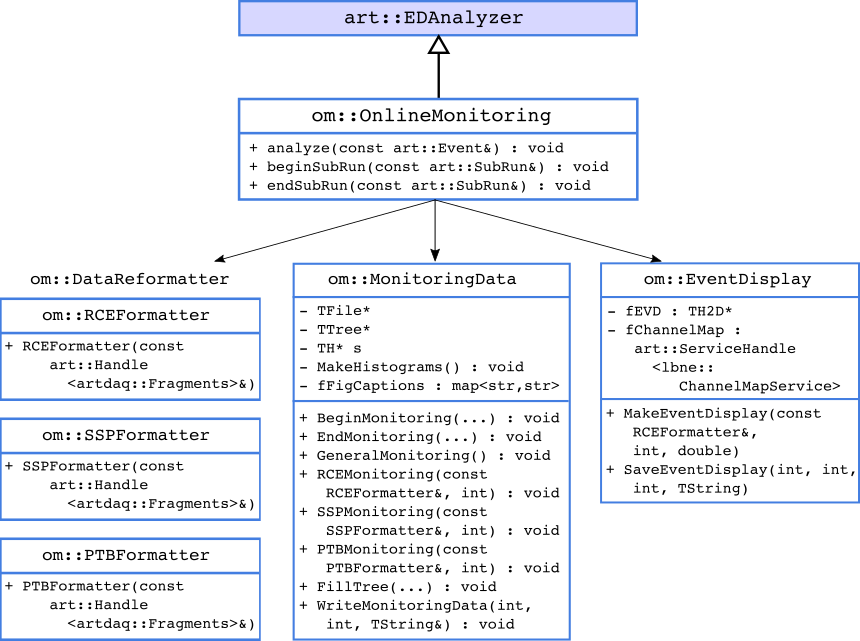
\includegraphics[width=12cm]{onlineMonitoringFramework.png}
  \caption{Demonstration of the framework designed for online monitoring in the DUNE 35ton experiment.}
  \label{fig:OnlineMonitoringFramework}
\end{figure}

\subsection{Monitoring Framework Design}\label{sec:MonitoringFrameworkDesign}

The setup consists of a central `module', \texttt{OnlineMonitoring\_module.cc}, which is configured within the art framework through its base class.  The OnlineMonitoring class controls the running of the system and owns instances of further classes, each designed for a specific purpose, controlling the data flow by calling the relevant methods when required.  Once an event has been obtained, the data for each component is processed and repackaged into RCEFormatter, SSPFormatter and PTBFormatter objects.  The purposes of this method are thus:
\begin{itemize}
\item to provide an interface between the raw data and the methods which analyse the data.  This is important as it provides a single point of maintainance for when formats change and allow for various `DAQ modes` to use the same analysis code;
\item to separate interaction with the DAQ from the handling of data objects;
\item to allow for jumping around the data for more detailed data analysis which would not be possible if just looking though the data linearly.
\end{itemize}
The main drawback to performing this step is it requires all the data to be held in memory until the end of the event and represents basically the same information as initially present.  However, it was decided the advantages were worth the compromises in memory useage required and no problems were apparent during the course of the run except when operating at the very limits of the capability of the DAQ.

These reformatted data objects are then passed to the methods in the MonitoringData class for straight forward anaylsis.  This class owns all of the data products which are output from the monitoring (e.g. histograms, graphs, trees and files) and deals with their filling and writing out when required.  This is discussed further in Sec. \ref{sec:DQM}.

The event display is handled by its own dedicated class, EventDisplay; this has methods for making the displays and saving them as an image in the correct place when required.  It is designed to accept the reformatted RCE object and presents the data in as meaningful way as possible; this is detailed fully in Sec. \ref{sec:EventDisplay}.

\subsection{Writing Monitoring Data}\label{sec:WritingMonitoringData}

The data objects are created new for each subrun and are written out at three points during data taking:
\begin{itemize}
\item an initial write out N seconds after the start of the subrun;
\item at frequent intervals during the subrun, every M seconds;
\item at the end of the subrun.
\end{itemize}
The parameters N and M are user defined and were set to 30 and 500 resepectively for normal data taking.  The data products are only cleared at the end of a subrun, so any intermediate writing out of data simply refreshes the current plots.

The event displays are computationally expensive to make and so were only created once per subrun during normal running.  However, since a subrun was automatically stopped by the DAQ and a new one started once the output file had reached 5 GB in size, and (since zero suppression was not utilised at any point during the run) this occurred on average every four minutes, a new event display was made every few minutes.

All the output data were saved on a shared disk on the gateway DAQ machines for further use.  This is discussed properly in Sec. \ref{sec:WebInterface} below.

\subsection{Configuring the Monitoring}\label{sec:MonitoringConfiguration}

[Possibly don't need this section...]
The system was designed to be flexible and many parameters were available to control the running of the monitoring.  These are listed and described below, with default parameter provided in brackets.

\begin{itemize}
\item TPCModuleLabel (``daq'') -- art module label for TPC data saved in the DAQ;
\item PhotonModuleLabel ([ ``sparseSsp'', ``daq'' ]) -- art module label for photon data saved in the DAQ;
\item TriggerModuleLabel (``daq'') -- art module label for counter data saved in the DAQ;
\item DetailedMonitoring (false) -- fills more, and usually more computationally expensive, data;
\item ScopeMonitoring (false) -- support for a different DAQ running mode, `scope mode';
\item DataDirPath (``/storage/data/'') -- path at which the data files are saved by the first aggregator;
\item MonitorSavePath (``/data2/lbnedaq/monitoring/'') -- location to save DQM data;
\item EVDSavePath (``/data2/lbnedaq/eventDisplay/'') -- location to save event displays;
\item PedestalFile (``/data2/lbnedaq/pedestal.csv'') -- location of the most recent pedestal file, containing pedestals for all channels.  This was used for pedestal subtraction when making event displays;
\item ImageType (``.png'') -- the format to save any images;
\item MonitoringRefreshRate (500) -- how often to write out the most recent monitoring data plots;
\item InitialMonitoringUpdate (30) -- how long after starting a new subrun to initially write out the data;
\item EventDisplayRefreshRate (60) -- how often to refresh the event display when not just making one per subrun;
\item LessFrequentFillRate (20) -- how often to fill the more computationally expensive plots;
\item DriftVelocity (0.9 \#mm/us) -- rough drift electron velocity, used for calculating the x coordinate for the event display;
\item CollectionPedestal (550) -- the default pedestal value if the file isn't readable;
\item MicroslicePreBuffer (5) -- how many microslices are saved by the RCEs before the one containing the trigger;
\item MicrosliceTriggerLength (5) -- the length of the trigger.
\end{itemize}

\section{Data Quality Monitoring}\label{sec:DQM}



\section{Online Event Display}\label{sec:EventDisplay}

One of the highlights of being in ROC West (Remote Opertation Control room at FNAL) during data taking was watching the online event display refresh with updated images representing cosmics passing through the detector.  Watching tracks appear in the data represented such a hugh acheivement for the DUNE 35ton operations team it never failed to cause excitement every time a new event appeared.  The event display also allowed for an incredibly straight forward way of monitoring the data -- high noise states, poor LAr purity and drift field problems were all immediately evident from the display.

Given the way in which data were read out of the detector, it proved challenging finding a way to represent this in a simple way that was comprehensible.  The construction of such a display is the subject of this section.

\section{Selecting the Data}\label{sec:SelectingEVDData}

[The data format will likely be described in the 35ton section -- most of this will probably be moved up to that point and referenced at a later stage...]

[I need to make a diagram showing this.] The raw format for the TPC data is complicated and has many levels of structure.  The 2048 channels are readout out by 16 front end boards (containing the cold electronics, including the digitisers), each processed by an RCE and then read into the DAQ by a board reader.  The format at this point is referred to as a millislice; there is a millislice for each of the detector components (RCEs, SSPs and PTB) and an `event' is a collection of all such millislices.  For the TPC data, a millislice contains all the information for 128 channels.  This data also has further substructure; a millislice is composed of N microslices, with each microslice containing M nanoslices.  A nanoslice contains 128 ADC values, representing one `tick' (== $500$ ns) worth of data for 1/16th of the detector.  A microslice thus contains this information for a `drift window' (M ticks) and a millislice a collection (M) of drift windows.  For the normal data running, N was set to 20 and M 1000.

As the detector collects data, the RCEs continually create and save microslices to send to the DAQ to form a millislice.  These microslices are empty (contain no nanoslices) until a trigger is received, at which point nanoslices are made and saved within each microslice.  There is also a buffer in place to save a certain number of full microslices (microslices containing nanoslices) before the microslice containing the trigger.  A certain number of full microslices proceeding the trigger are also recorded by the RCEs.  During normal running, a `$4+1+10$' format was employed; four microlices containing nanolices before the trigger was recieved, the microslice containing the trigger, and the ten following microslices.  It should be further noted that, since the DAQ was designed for continuous data readout, these microlices need not necessarily be within the same millislice: it is possible for the trigger to occur in microslice 18 of a certain millislice, meaning the 15 filled microslices will straddle successive millislices.  This is demonstrated in Fig. \ref{fig:MicrosliceTrigger}.

\begin{figure}[ht]
  \centering
  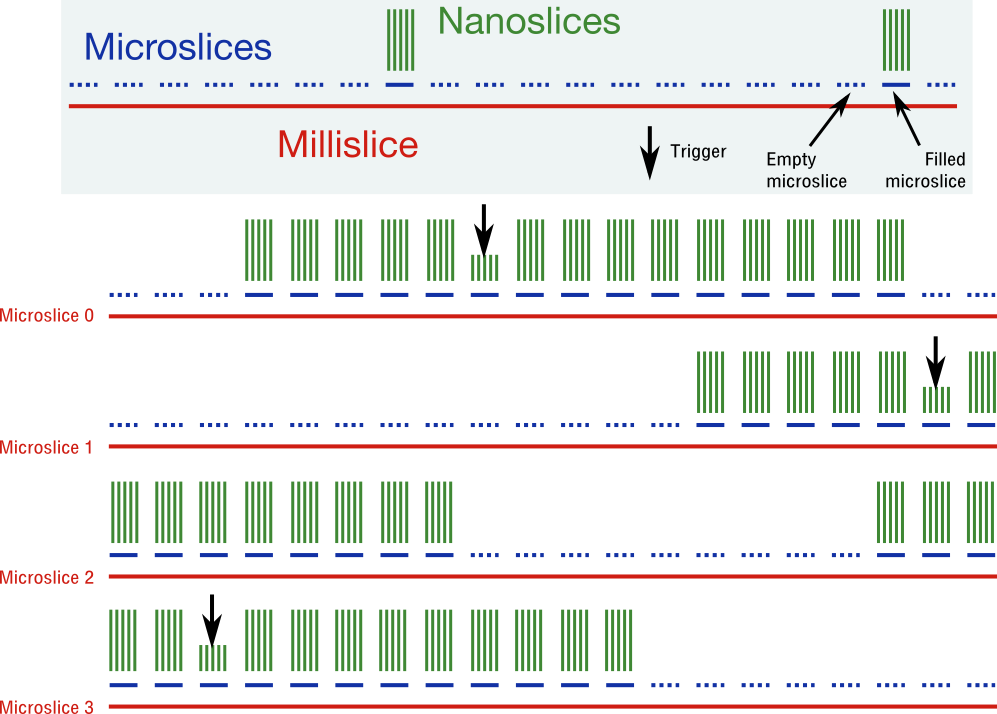
\includegraphics[width=16cm]{microsliceTrigger.png}
  \caption{Demostration of how TPC data is saved when using a DAQ designed for continuous readout.  The black arrows represent hypothetical triggers occurring within the duration of a particular microslice.  In each case, the 4 preceeding microslices and the 10 proceeding microslices are filled with nanoslices and saved; all other microslices are saved with no nanoslices since they contain no useful data.  An example of such an event is shown occurring in Microslice 0 in the figure.  As described in the text, a trigger can cause the useful microslices to straddle consequetive millislices; this is represented in the following microslices in the figure.}
  \label{fig:MicrosliceTrigger}
\end{figure}
Note this also results in real `physics events' being saved in separate `DAQ events'; for this reason a splitter/stitcher module has been designed to extract the actual triggered events from the raw data and repackage them into a useful event structure -- this is the first stage before all offline analysis with the 35ton data.

Since the event display runs online, a subtle selection must be applied to ensure the full physics event occurs within the current DAQ event; proceeding and preceeding events are unaccessible to the DAQ during running.  This is achieved by noting whether or not a trigger occurred (i.e. microslices contain nanoslices) when reformatting the RCE data in DataReformatter, and which microslice it occurred in.  For the event display, a triggered event is only useful if the trigger occurred within a certain range (e.g. microslice 5 to microslice 10); this ensures all the filled microslices are present within the current millislice.  The event displayed is then filled for a given range of microslices around the trigger to capture all the actual physics data.

\subsection{Representing the Data}\label{RepresentingEVDData}

Due to the wrapped nature of the induction wires in the 35ton, and disambiguation impossible without full reconstruction, it makes little sense to look at charge deposited on these planes.  This results in only the collection planes being useful for showing the data in this way, meaning just one dimension.  A second dimension is possible if the view is changed to show a representation of the TPC from above and use drift time as a second dimension.  This requires the two centre APAs be shown together as one combined readout structure.  A `global collection wire' is defined by numbering the wires across the APAs, leaving a space for the gaps inbetween, and used to represent the dimension across the TPC.  The drift time, in ticks, represents the second spacial coordinate once charge collected in the short drift volume has been corrected to a negative tick.

By working with the system used to record pedestal values of the channels, it is possible to perform an approximate pedestal subtraction on the data.  Whenever a pedestal run is performed by a shifter, a text file containing all the calculated pedestal values for each channel is created and subsequently uploaded to a database for offline use.  By making sure a copy of the most recent pedestal file is always available to the monitoring framework, it is possible to always represent the charge as accurately as possible.  It is then ensured the pedestal-subtracted ADC values are within the range $0-250$ to limit the noisy channels and correct for any accidental negative charge.  Finally, given the relatively low signal-to-noise ratio, it was decided a greyscale image showed the best resolution for seeing tracks traverse the cryostat.

An example event display is shown in Fig. \ref{fig:EVD}.

\begin{figure}
  \centering
  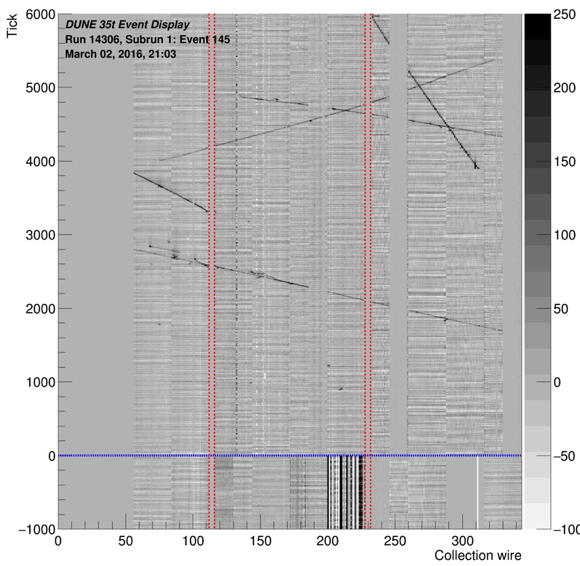
\includegraphics[width=14cm]{evd.png}
  \caption{Example online event display made as part of the online monitoring framework for run 14306 (2nd March, 2016).  The view is from the top of the detector looking down; the red lines represent the spaces between the APAs and the blue line the location of the APA frames, separating the long and short drift regions.}
  \label{fig:EVD}
\end{figure}

\section{Monitoring Web Interface}\label{sec:WebInterface}

